\documentclass{article}
\usepackage{tikz}

\begin{document}
\centering

\begin{tikzpicture}[scale=1.2]

\tikzset{
  lattice node/.style={
    inner sep=2pt,
    outer sep=2pt,
  }
}

% Level 0
\node[lattice node] (bot) at (0,0) {$\bot$};

% Level 1 (shifted up more)
\node[lattice node] (a) at (-2,2) {$a$};
\node[lattice node] (b) at (0,2)  {$b$};
\node[lattice node] (c) at (2,2)  {$c$};

% Level 2 (more vertical spacing)
\node[lattice node] (ab) at (-2,4) {$a \vee b$};
\node[lattice node] (ac) at (0,4)  {$a \vee c$};
\node[lattice node] (bc) at (2,4)  {$b \vee c$};

% Level 3 (top element higher still)
\node[lattice node] (top) at (0,6) {$\top$};

% Edges
\draw (bot) -- (a);
\draw (bot) -- (b);
\draw (bot) -- (c);

\draw (a) -- (ab);
\draw (a) -- (ac);
\draw (b) -- (ab);
\draw (b) -- (bc);
\draw (c) -- (ac);
\draw (c) -- (bc);

\draw (ab) -- (top);
\draw (ac) -- (top);
\draw (bc) -- (top);

\end{tikzpicture}

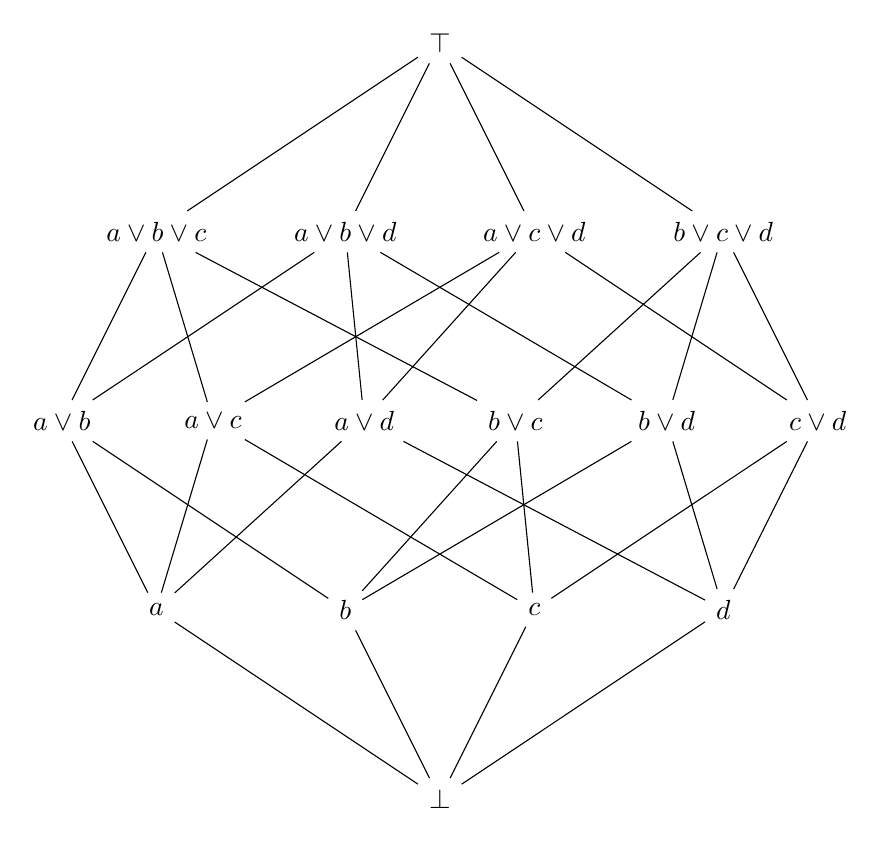
\begin{tikzpicture}[scale=1.2]

\tikzset{
  lattice node/.style={
    inner sep=2pt,
    outer sep=2pt,
  }
}

% Level 0
\node[lattice node] (bot) at (0,0) {$\bot$};

% Level 1: atoms (4 nodes)
\node[lattice node] (a) at (-3,2) {$a$};
\node[lattice node] (b) at (-1,2) {$b$};
\node[lattice node] (c) at (1,2)  {$c$};
\node[lattice node] (d) at (3,2)  {$d$};

% Level 2: 2-element joins (6 nodes, perfectly symmetric)
\node[lattice node] (ab) at (-4.0,4) {$a \vee b$};
\node[lattice node] (ac) at (-2.4,4) {$a \vee c$};
\node[lattice node] (ad) at (-0.8,4) {$a \vee d$};
\node[lattice node] (bc) at (0.8,4)  {$b \vee c$};
\node[lattice node] (bd) at (2.4,4)  {$b \vee d$};
\node[lattice node] (cd) at (4.0,4)  {$c \vee d$};

% Level 3: 3-element joins (4 nodes)
\node[lattice node] (abc) at (-3,6) {$a \vee b \vee c$};
\node[lattice node] (abd) at (-1,6) {$a \vee b \vee d$};
\node[lattice node] (acd) at (1,6)  {$a \vee c \vee d$};
\node[lattice node] (bcd) at (3,6)  {$b \vee c \vee d$};

% Level 4: top
\node[lattice node] (top) at (0,8) {$\top$};

% Edges bottom -> atoms
\draw (bot) -- (a);
\draw (bot) -- (b);
\draw (bot) -- (c);
\draw (bot) -- (d);

% Edges atoms -> 2-element joins
\draw (a) -- (ab);
\draw (a) -- (ac);
\draw (a) -- (ad);

\draw (b) -- (ab);
\draw (b) -- (bc);
\draw (b) -- (bd);

\draw (c) -- (ac);
\draw (c) -- (bc);
\draw (c) -- (cd);

\draw (d) -- (ad);
\draw (d) -- (bd);
\draw (d) -- (cd);

% Edges 2-element -> 3-element joins
\draw (ab) -- (abc);
\draw (ac) -- (abc);
\draw (bc) -- (abc);

\draw (ab) -- (abd);
\draw (ad) -- (abd);
\draw (bd) -- (abd);

\draw (ac) -- (acd);
\draw (ad) -- (acd);
\draw (cd) -- (acd);

\draw (bc) -- (bcd);
\draw (bd) -- (bcd);
\draw (cd) -- (bcd);

% Edges 3-element -> top
\draw (abc) -- (top);
\draw (abd) -- (top);
\draw (acd) -- (top);
\draw (bcd) -- (top);

\end{tikzpicture}




%%%%%%%%%%%
Three-atom case with some uniform probabilities:
\begin{tikzpicture}[scale=1.2]

\tikzset{
  lattice node/.style={
    inner sep=2pt,
    outer sep=2pt,
  }
}

% Level 0
\node[lattice node] (bot) at (0,0) {$0$};

% Level 1 (shifted up more)
\node[lattice node] (a) at (-2,2) {$\frac{1}{3}$};
\node[lattice node] (b) at (0,2)  {$\frac{1}{3}$};
\node[lattice node] (c) at (2,2)  {$\frac{1}{3}$};

% Level 2 (more vertical spacing)
\node[lattice node] (ab) at (-2,4) {$\frac{1}{6}$};
\node[lattice node] (ac) at (0,4)  {$\frac{1}{6}$};
\node[lattice node] (bc) at (2,4)  {$\frac{1}{6}$};

% Level 3 (top element higher still)
\node[lattice node] (top) at (0,6) {$1$};

% Edges
\draw (bot) -- (a);
\draw (bot) -- (b);
\draw (bot) -- (c);

\draw (a) -- (ab);
\draw (a) -- (ac);
\draw (b) -- (ab);
\draw (b) -- (bc);
\draw (c) -- (ac);
\draw (c) -- (bc);

\draw (ab) -- (top);
\draw (ac) -- (top);
\draw (bc) -- (top);

\end{tikzpicture}




\end{document}
